\section{Introduction}

PDF is a widely accepted format for sharing and presenting documents, as it ensures that the layout and formatting of the document remain consistent across different devices and operating systems. This is particularly important in scientific publications, where complex figures, tables, and equations need to be accurately represented.
PDFs are designed for documents intended for printing, as they can embed fonts and high-quality images, and scientific journals traditionally required high-resolution print-ready files for publication. 
PDFs files can be signed digitally, providing a level of security and authenticity for scientific publications. This is important to ensure the integrity and trustworthiness of research findings, particularly in fields where reproducibility and transparency are paramount.
Although isolating trends in the Internet jungle is challenging, PDF documents account for about 85\% of the Common Crawl dataset\footnote{\url{https://commoncrawl.github.io/cc-crawl-statistics/plots/mimetypes}} and interest has been growing\footnote{\url{https://trends.google.com/trends/explore?date=2000-01-01\%202024-01-19&q=PDF}}. 
However, it is important to note that, while PDF has been widely used in scientific publications, there are emerging trends and technologies that challenge its status as a "de facto" format. For example, the rise of open-access publishing has led to the adoption of HTML and XML formats for online articles, allowing greater interactivity, accessibility, and searchability of scientific content.
However, those formats are penalised by the lack of standardised approaches, leading to a jungle of flavours of the same original format (e.g., JATS is one of the most widely used).

\section{Proposed approach}

Given the important role of PDF documents in the dissemination of scientific knowledge, supporting them natively is a necessary step to build effective TDM processes. 
In our approach, we use the Grobid library (Generation of Bibliographic Data)~\cite{Grobid}, which provides the ability to parse and structure text from PDF documents, such as scientific publications or patents. 
Grobid implements a set of pre-trained models supporting different architectures, including Conditional Random Field (CRF)~\cite{lafferty2001conditional}, Recurrent Neural Networks~\cite{lample2016neural}, and transformer-based~\cite{devlin2018bert}.
There are other tools for similar tasks, such as Cermine~\cite{tkaczyk2015cermine}, ParsCit~\cite{councill2008parscit}, however, Grobid was the highest-performing out-of-the-box tool~\cite{tkaczyk2018evaluation}.
Grobid has been successfully extended to support several domain-specific problems, for example, recognition of astronomical entities~\cite{grobid-astro}, segmentation of dictionaries~\cite{khemakhem2017automatic}, software mention~\cite{software-mentions}. 
Among the various open-source tools available, at the time of writing, it is still actively developed and used in several large-scale research repositories, such as Mendeley~\cite{mendeley-extraction}, ResearchGate (\url{https://researchgate.com}), Scite.ai (\url{https://www.scite.ai})~\cite{nicholson2021scite}. 

Grobid offers several advantages. 
a) It does not require one to make multiple agreements with different publishers to obtain source documents. A growing number of open-access pre-print repositories offer a viable alternative for gathering input data. 
b) PDF support in Grobid allows one to focus on the processing of a single format instead of dealing with several XML flavours. 
c) It is integrated with PDFAlto (\url{https://github.com/kermitt2/pdfalto}), a specialised tool for converting PDF to XML, which mitigates extraction issues such as invalid character encoding and incorrectly ordered text flow. PDFAlto supports the resolution of embedded fonts and layout variants such as multi-column. 
d) The Grobid internal data model \textit{LayoutTokens} access information in PDF documents at a low level for each token: style (italic, bold, superscript, and subscript), font (font type, font size), and coordinates within the visual document. 
e) By parsing PDF format natively, Grobid gives access to full text, figures, tables, and thus does not limit our work to public information such as abstracts.
Finally, f) Grobid includes a set of high-quality out-of-the-box pre-trained machine learning models.

In this contribution and in the following contributions, we introduce Grobid-superconductors, a novel application of the Grobid library as a text mining pipeline for scientific publications in materials science.
Our approach differs from other related works in several aspects. 
1) Instead of abstracts~\cite{mitsui2023automatic}, we support extraction from full-text body.
2) There is no requirement for us to reach an agreement with publishers~\cite{kononova2019text}.
3) We focus on processing a single format instead of dealing with several XML flavours~\cite{kononova2019text}
4) We avoid web scraping~\cite{court2020magnetic} and other processes that require addressing each website differently and requiring to update regularly to follow potential changes in the websites.
5) We use low-level layout details as attributes in our machine learning models that handle intricate representations of materials. For instance, the inclusion of superscripts or subscripts (which may not always be present in XML-formatted documents provided by publishers) can be intuitively advantageous in identifying chemical formulas.

\subsection{Publisher's agreement for source data}
Obtaining scientific articles through publisher APIs (Application Programming Interface) or web scraping can be inconvenient for several reasons. 
Many publishers control access to their API, demanding subscriptions or pay-per-view models, limiting accessibility for those without institutional access or financial means. 
API limitations, such as the number of requests allowed within a specific time frame, can slow down data retrieval, especially with a large volume of articles. The lack of standardisation in metadata and content formatting further complicates the extraction process.
As we have mentioned before, each publisher provides its own "JATS-flavoured standard", making it challenging to create a standardised data set from multiple sources. 
However, web scraping does not guarantee any data format stability and may breach the publisher's terms of service, leading to legal and ethical complications.
Open access resources, including institutional repositories and pre-print servers, offer a wealth of scientific literature at a reduced cost and in a consistent PDF format that represents a convenient means to access and process articles from these sources due to their accessibility and lack of legal constraints.

\subsection{Abstract versus full-text}
The abstract of a scientific paper, a concise summary located at the beginning of the document, serves as a quick overview that summarises the objectives, methods, results, and conclusions of the research in 150 to 250 words. 
Researchers frequently employ abstracts to assess the relevance of a paper to their work and for streamlined database searches. 
In contrast, the full text of a scientific article delves into comprehensive details, spanning sections such as introduction, methodology, results, discussion, and conclusions. This exhaustive account is crucial for in-depth literature reviews, detailed analysis of methodology, data review, and evaluation of the validity of conclusions.
Taking into account the perspective of TDM, both abstracts and full-texts play distinct roles. Abstracts, due to their succinct nature, are suitable for large-scale automated analyses, offering rapid insights into trends, topics, or keywords across a multitude of papers. However, full texts are amenable to more in-depth TDM, allowing for detailed extraction of information and revealing nuanced relationships between concepts, methodologies, and findings. 
Although previous studies~\cite{yamaguchi-etal-2020-sc} have used abstracts, our research focusses on extracting complex information from scientific documents using the entire fulltext.


\section{TDM pipeline}
\label{subsubsec:document-structuring}

Our TDM pipeline is built as a Grobid module called Grobid-superconductors. 
Grobid-superconductors is structured as a three-step process illustrated in Figure~\ref{fig:pipeline-overview}. The input is a PDF document which is converted to an internal model composed of text passages, tokens, and features. Those three elements are then used to perform Named Entities Recognition (NER), which are then linked by a Relation Extraction (RE) process. 
The output is a structured object serialised in JSON format.

\begin{figure}[htbp]
    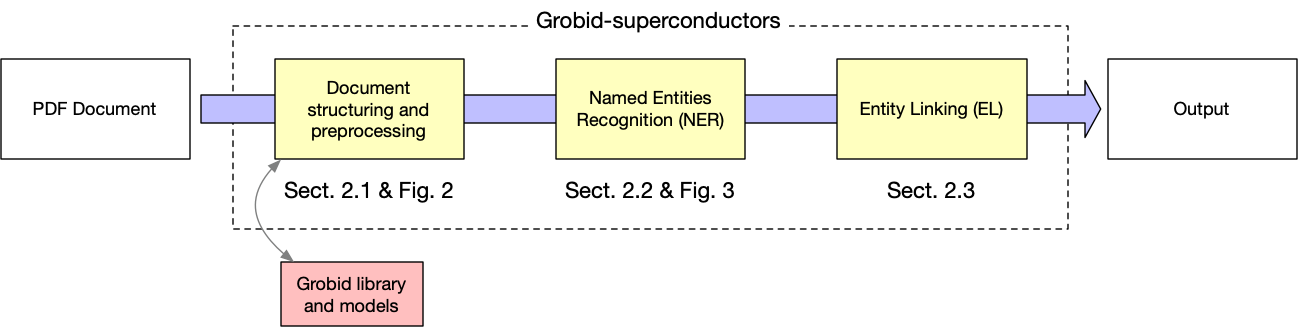
\includegraphics[width=\textwidth]{figures/automatic_extraction_supercon/schema-architecture-colors.png}
    \caption{Processing pipeline for extracting superconductors materials and properties. }
    \label{fig:pipeline-overview}
\end{figure}

\subsection{Document structuring and segmentation}

The initial stage of our procedure involves using Grobid and PDFAlto to convert the PDF document. This results in the segmentation of raw data into a basic structure consisting of header, body, and annexes using the \emph{Segmentation ML model}.
These three structures are then parsed by a second Grobid model \emph{Fulltext ML model} that identify paragraphs, section heads, and references for body and annexes. 
We have created a custom process that analyses the structure and generates an internal model based on a list of text statements, tokens, and features. For example, the content of the tables is excluded, but the table captions are retained.
In the process, we can also assign \textit{section} and \textit{subsection} information, as the results of the Grobid first level: header, body, and annex, and the second level (paragraph, table or figure caption, abstract, title) structures.

Header structures are parsed with the \emph{Header ML model} to identify bibliographic data. 
This aggregated version only includes information that is relevant to our TDM process. 
Our process selects a subset of bibliographic information from the header: title, authors, DOI, publisher, journal, and year of publication, and we consolidate them via Grobid to match the publisher's quality (even by processing the ``pre-print version'' of the publication).

\begin{figure}[htbp]
    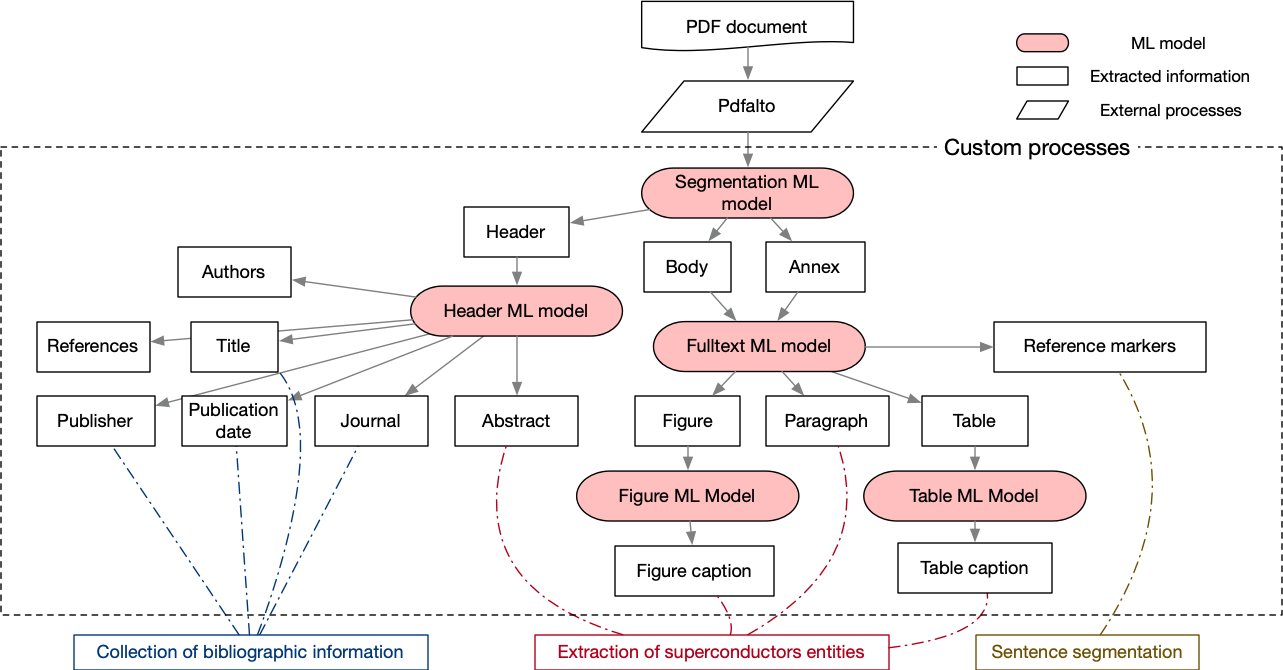
\includegraphics[width=\textwidth]{figures/automatic_extraction_supercon/document-structuring-colors}
    \caption{Grobid-superconductors extraction processes (bibliographic information, superconductor entity extraction and sentence segmentation) within the Grobid cascade data flow.}
    \label{fig:grobid-document-processing}
\end{figure}

\subsection{Sentence segmentation}
% Sentences vs Paragraphs 
An additional query concerning natural language processing (NLP) pertains to the choice between employing sentence-based or paragraph-based text.
While paragraphs can be extracted as part of the PDF document's layout, obtaining sentences requires an additional step through a sentence segmenter. Sentences are typically shorter, which offers advantages in processing with large deep learning models.
During training, sentences use less memory and allow us to train models with a larger ``batch size'', which has been shown to improve efficiency and obtain better results~\cite{liu2019roberta}. 

\begin{table}[ht]
    \centering
    \caption{Results from cross-validation for sentence-based and paragraphs-based text. Measurements are micro average. P: Precision, R: Recall, and F1: F1-score.}
    
    \begin{tabular}{lccc}
        \toprule
        \textbf{Label}   & \textbf{P}   & \textbf{R}    & \textbf{F1} \\
        \midrule
        Paragraph-based  & 44.44        & 27.21         & 33.76       \\
        Sentence-based   & 48.41        & 50.00         & 51.70       \\
        \bottomrule
    \end{tabular}

    \label{tab:comparison-evaluation-sentences-paragraphs}
\end{table}

We chose to use sentence-based segmentation in Grobid-superconductors after performing small-scale preliminary experiments on our task. 
For the Named Entities Recognition (NER) task, we trained and evaluated a sequence labelling model for each approach (paragraph and sentence based) in four annotated documents (3/1 document partition for training/evaluation) from SuperMat, a dataset that we built~\cite{foppiano2021supermat} and is described in Chapter~\ref{cha:supermat}.
As indicated in Table~\ref{tab:comparison-evaluation-sentences-paragraphs}, the F1 score increased by 17.94\% points when using sentence-based text.

For the RE task, we found in a previous study~\cite{foppiano2019proposal} that the sentence-based approach would favour higher precision, while the paragraph-based approach would result in greater recall.
% Therefore, we establish that a sentence-based approach is more beneficial than a paragraph-based approach for our tasks.

Since Grobid supports partitioning documents down to the paragraphs, a sentence segmenter is necessary. The problem has been long investigated~\cite{sadvilkar2020pysbd,loper2002nltk,neumann2019scispacy,gillick2009sentence,read2012sentence,spacy2,bling2020}, however, there are still challenges in segmenting paragraphs from scientific text: reference reference markers (also called \textit{reference callouts}), formnulas, and other constructs may contain periods and mislead algorithms. 
Thanks to Grobid and the ability to recognise reference markers and formulas, we use the collected ones from the text as features to improve paragraph segmentation in sentences: segmentation is aborted if the end of a sentence falls within the boundaries of one of these markers.
For example, a sentence such as "\textit{[...]The evaluation from (2021, Foppiano et al.) offers a solid validation for our method}" containing a reference in the form ``(2021, Foppiano et al.)'' and may be mistakenly segmented in the middle token ``[...] et al.'' and the new sentence starts with ``) offsers [...]''. 

\section{Conclusions}

In conclusion, the application of innovative techniques, exemplified by Grobid, marks a significant milestone in the field of materials science. This effort represents a novelty for the first integration of such methods within the domain, showcasing the potential for transformative advancements. 
By sidestepping the complexities and expenses associated with signing agreements with scientific publishers and the intricate landscape of XML formats, this approach not only streamlines the dissemination process, but also liberates researchers from the often daunting challenges posed by conventional publishing models.

In the evolving landscape of scientific dissemination, where alternative means gain traction, it is noteworthy that the PDF format remains resilient as the "de facto" standard. The decision to publish through open access aligns with the current trend toward greater accessibility and openness in scholarly communication. 
The increasing availability of open-access articles further reinforces the utility and relevance of Grobid, positioning it favourably as a valuable tool in the arsenal of researchers seeking efficient and cost-effective methods for sharing scientific knowledge in the materials science domain.

In this contribution, we introduced grobid-superconductors, and we described the component responsible for reading and structuring PDF documents, preparing the data to be processed by our novel specialised models which are discussed in Chapters~\ref{cha:extraction-experimental-data} and~\ref{cha:measurements}.

This contribution was published as part of the paper "Automatic extraction of materials and properties from scientific literature"~\cite{foppiano2023automatic}.